\section{Problemstellung} \label{sec:Problemstellung}

Die zentrale Herausforderung bei der Entwicklung von Stadtmetaphern zur Softwarevisualisierung besteht in der Festlegung eines geeigneten Layouts für die Visualisierung. Im Abschnitt \ref{sec:CodeCity} wurde das ursprüngliche Layout-Konzept der CodeCity-Analogie vorgestellt. Ein gemeinsames Grundprinzip dieser und verwandter Arbeiten ist, dass zunächst ein 2D-Layout erzeugt wird, das anschließend durch eine zusätzliche Metrik in die dritte Dimension extrudiert und schließlich durch weitere Metriken (z.B. Farbe, Transparenz) angereichert wird.
In dieser Arbeit werden wir uns genau auf dieses Grundprinzip konzentrieren und untersuchen, wie sich verschiedene Layout-Algorithmen auf die Visualisierung von Code-Qualitätsmetriken auswirken.
Die daraus entstehende Leitfrage lautet:

\begin{quote}
Welches Layout eignet sich am besten zur Visualisierung von Code-Qualitätsmetriken? Gibt es Ansätze, die Übersichtlichkeit und Verständlichkeit im Vergleich zu bestehenden Lösungen (insbesondere der CodeCity-Metapher) verbessern?
\end{quote}

Daraus ergeben sich für diese Arbeit folgende konkrete Forschungsfragen:
\begin{enumerate}
    \item Wie lassen sich bestehende Treemap-Layout-Algorithmen an das spezifische Anwendungsproblem dieser Arbeit anpassen? Welche Vor- und Nachteile resultieren daraus?
    \item Lassen sich durch Analyse verwandter Arbeiten und bestehender Tools alternative Layouts identifizieren, die eine bessere Grundlage für die Visualisierung von Code-Qualitätsmetriken bieten? 
    \begin{enumerate}
        \item Beispielhaft: Übertrifft das Sunburst-Layout das beste Treemap-Layout im Hinblick auf die Darstellung von Code-Qualitätsmetriken?
        \item Beispielhaft: Bietet das Stack-Layout Vorteile gegenüber klassischen Treemap-Layouts für diesen Anwendungszweck?
    \end{enumerate}
\end{enumerate}

\subsection{Evaluationsrahmen} \label{sec:Evaluationsrahmen}

Um die angestrebten Visualisierungen eindeutiger zu evaluieren und in ihrem Ziel klarer zu definieren, orientieren wir uns an den fünf Dimensionen der Softwarevisualisierung nach Marcus Adrian et al. \cite[2]{3dsoftwareMarcus}:
\begin{quote}
    \begin{itemize}
        \item \textbf{Tasks}: Warum wird die Visualisierung benötigt?
        \item \textbf{Audience}: Wer nutzt die Visualisierung?
        \item \textbf{Target}: Welche Datenbasis/Quelle wird abgebildet?
        \item \textbf{Representation}: Wie wird die Information dargestellt?
        \item \textbf{Medium}: Wo findet die Darstellung statt?
    \end{itemize}
\end{quote}

\subsubsection*{1. Warum ist die Visualisierung von Code-Qualitätsmetriken wichtig?}
Die Visualisierung von Code-Qualitätsmetriken ermöglicht die Bewertung und das bessere Verständnis der Softwarequalität. Sie dient dazu, einen schnellen Überblick über komplexe Codebasen zu erhalten, Hotspots zu identifizieren und vertiefende Analysen effizient einzuleiten. Besonders wichtig ist es dabei, Zusammenhänge zwischen verschiedenen Metriken auf einen Blick erfassbar zu machen, was in rein tabellarischer oder isolierter Darstellung kaum möglich ist. Das Hauptziel besteht darin, das abstrakte Konzept der Codequalität \textit{greifbar} und anschaulich zu machen.

\subsubsection*{2. Wer ist die Zielgruppe der Visualisierung?}
Die Visualisierung richtet sich primär an Personen ohne tiefgehende Kenntnisse der Codebasis und ohne Programmierkenntnisse. Trotzdem kann die Visualierung aber auch Entwicklerinnen und Entwicklern helfen, die sich neu in ein Projekt einarbeiten oder Teams, die systematisch die Softwarequalität verbessern wollen, in der Kommunikation unterstützen.

\subsubsection*{3. Was ist die Datenquelle?}
Grundlage sind hierarchische Code-Qualitätsmetriken, die automatisiert aus dem Source Code extrahiert werden. Jeder Knoten der Hierarchie (Node) besitzt dabei einen Namen und entweder eine Liste von Kindknoten (children) oder einen Wert (value), der die Metrik repräsentiert (siehe Listing \ref{lst:nodeSchema}). 
Diese Struktur ermöglicht es, komplexe Softwareprojekte in übersichtliche Hierarchien zu zerlegen, die dann visualisiert werden können.

\begin{lstlisting}[language=json, caption={Schema einer Node}, label={lst:nodeSchema}]
    "node": {
        "name": string,
        "children": List[Node] | "value": number
    }
\end{lstlisting}

\subsubsection*{4. In welchem Medium soll die Visualisierung erfolgen?}
Die Visualisierung ist für die digitale Darstellung auf herkömmlichen Bildschirmmedien konzipiert. Im vorliegenden Prototyp wird eine Umsetzung im Webbrowser mittels TypeScript und Three.js realisiert. Die Übertragung der Methoden auf andere Programmierumgebungen ist möglich.

\subsubsection*{5. Wie erfolgt die Darstellung?}
Das Visualisierungskonzept lehnt sich an den in den Grundlagen erläuterten Stadtmetapher-Ansatz an (Abschnitt \ref{sec:CodeCity}). Im Mittelpunkt dieser Arbeit steht das zweidimensionale Layout der Knoten. Die Gestaltung dieses Layouts wird jedoch eingeschränkt, dadurch, dass Fläche, Höhe und Farbgebung (auch Schattierung, Struktur oder Transparenz) zur Darstellung verschiedener Metriken dienen. Maßnahmen wie das Einfärben von verschiedenen Ordnern oder Modulen, zur besseren visuellen Unterscheidung fallen für die Visualisierung in dieser Arbeit weg. Stattdessen wird der Fokus auf die geschickte Platzierung, Wahl von Abständen und Beschriftung gelegt. 

\smallskip

Aus dem hier definierten Rahmen und den in den Grundlagen beschriebenen Grundlegenden Anforderungen (Abschnitt \ref{sec:3DSoftwareVisualisierung}) leiten sich für die, im Rahmen dieser Arbeit entwickelte, Visualisierung folgende Anforderungen ab:

\begin{itemize}
    \item \textbf{Informationsgehalt und effiziente Nutzung des Platzes:} Möglichst viel relevante Information soll bei minimalem Flächenverbrauch dargestellt werden.
    \item \textbf{Niedrige visuelle Komplexität und hohe Verständlichkeit:} Das Layout muss klar und intuitiv lesbar bleiben, um Überforderung zu vermeiden.
    \item \textbf{Skalierbarkeit:} Auch umfangreiche Softwaresysteme müssen übersichtlich visualisierbar sein.
    \item \textbf{Korrelation mit dem Code:} Eine gute Zuordnung zwischen Visualisierung und Source Code muss gewährleistet sein, um Rückschlüsse auf die Softwarestruktur zu ermöglichen.
    \item \textbf{Stabilität gegenüber Änderungen:} Nachrangig, aber erwünscht ist, dass die Visualisierung auf Änderungen im Code robust reagiert, um zeitliche Vergleiche zu ermöglichen, ohne dass der Betrachter sich neu orientieren muss.
\end{itemize}

\subsection{Das Treemap-Problem} \label{sec:TreemapProblem}

Durch die nähere Erlärung des Treemap-Algorithmus (siehe Abschnitt \ref{sec:Treemap}) wurde gezeigt, dass klassische Treemap-Algorithmen grundlegende Schwächen auf weisen, insbesondere wenn Abstände (\textit{Margins}) zwischen den Knoten dargestellt werden sollen. Das Grundproblem, das von Johnson und Shneiderman \cite{johnson1991tree} adressiert wurde, ist bereits ohne Abstände NP-Hard \cite[3]{bruls2000squarified}, und zusätzliche Abstände verkomplizieren die Problematik noch weiter.

Wesentliche Schwierigkeiten bei der Integration von Abständen in das Layout ergeben sich durch:
\begin{itemize}
    \item Die abgezogenen Flächen für Abstände führen dazu, dass die verbleibende Knotenfläche nicht mehr proportional zum Wert des Knotens ist.
    \item Bei kleinen Knoten können durch Abzüge von Minimalabständen einzelne Knoten ganz verschwinden, wenn ihre minimale Länge oder Breite kleiner als der geforderte Abstand wird.
\end{itemize}

In den Abbildungen \ref{fig:zeroMarginArtificialMap}, \ref{fig:fiveMarginArtificialMap} und \ref{fig:tenMarginArtificialMap} sind verschiedene Treemap-Layouts zu sehen, die mithilfe des Squarify-Algorithmus (siehe Abschnitt \ref{sec:Squarify}) erzeugt wurden. Die zugrundeliegenden Strukturen und Metriken wurden dabei händisch erstellt, um typische Probleme bei der Flächenproportionalität und Sichtbarkeit in Treemaps zu verdeutlichen (siehe Anhang \ref{lst:artificial.cc.json}).

In Abbildung \ref{fig:zeroMarginArtificialMap} sind alle Knoten sichtbar, und die Flächen allen Knoten sind proportional zu dem jeweiligen Wert. Dadurch ergibt sich eine exakte Flächenproportionalität zwischen Wert und Darstellung.

In Abbildung \ref{fig:fiveMarginArtificialMap} ist zwar weiterhin jeder Knoten sichtbar, jedoch sind die Flächen nicht mehr exakt proportional zu den Werten der Knoten. Beispielsweise besitzt der große Knoten 3 mit dem Wert 3000 nur noch eine Fläche von etwa 2600, was ein Flächen-Wert-Verhältnis von ungefähr 0,9 ergibt. Der kleine Knoten oben links (Knoten 5) mit dem Wert 30 weist hingegen nur noch eine Fläche von etwa 5 auf, entsprechend einem Verhältnis von ca. 0,2.  Knoten 2 hat eine Fläche von etwa 17, er erscheint also, obwohl er den selben Wert hat wie Knoten 5, deutlich größer. Dies verdeutlicht, dass die Abstände die Flächenproportionalität erheblich beeinträchtigen.

In Abbildung \ref{fig:tenMarginArtificialMap}, bei einem Abstand von 10, werden einige Knoten, zum Beispiel wie etwa der zuvor oben links gelegene Knoten 5 mit Wert 30, gar nicht mehr dargestellt, da ihre berechnete Breite kleiner als der vorgegebene Abstand ist. Damit sind relevante Informationen in der Visualisierung nicht länger sichtbar.

Diese Beispiele verdeutlichen die Auswirkungen gewählter Abstandsparameter auf Proportionalität und Lesbarkeit von Treemaps.

\begin{figure}
    \centering
    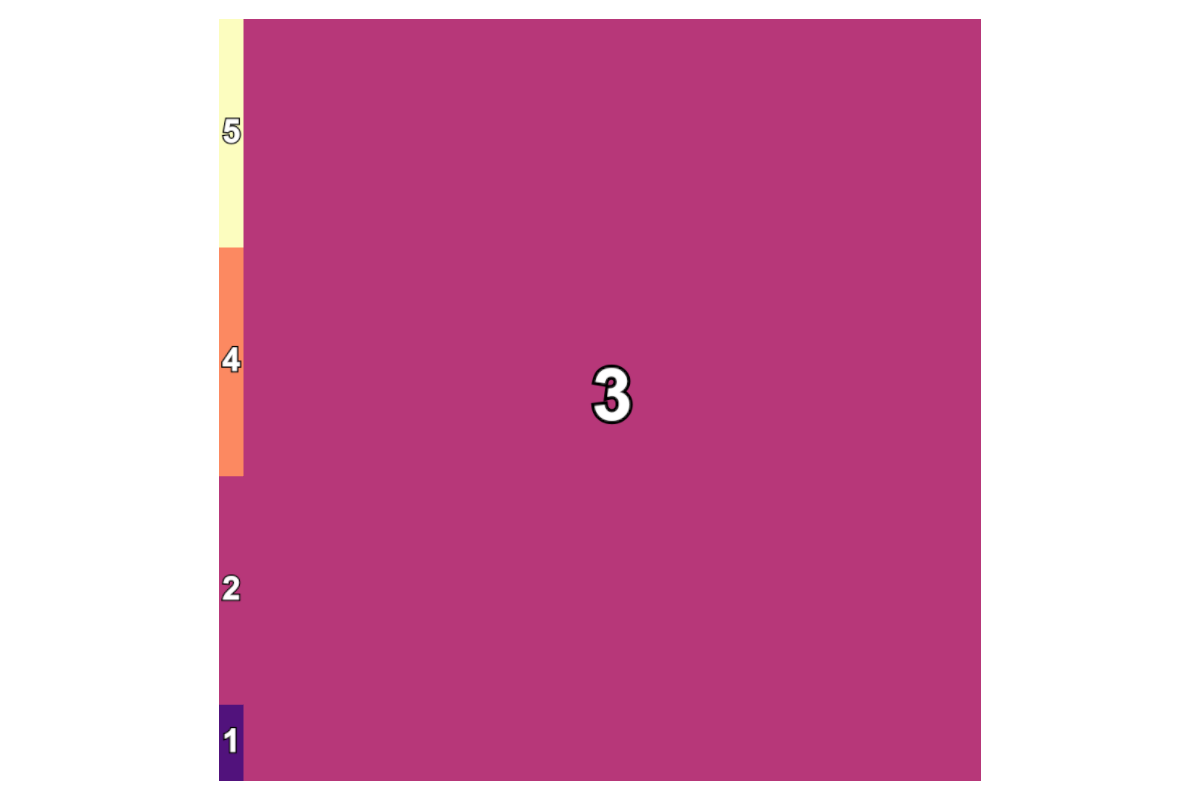
\includegraphics[width=0.8\textwidth]{images/zeroMarginArtificialMap.png}
    \caption{Treemap-Layout, generiert mit dem Squarify-Algorithmus (Abstand 0).} 
    \label{fig:zeroMarginArtificialMap}
\end{figure}

\begin{figure}
    \centering
    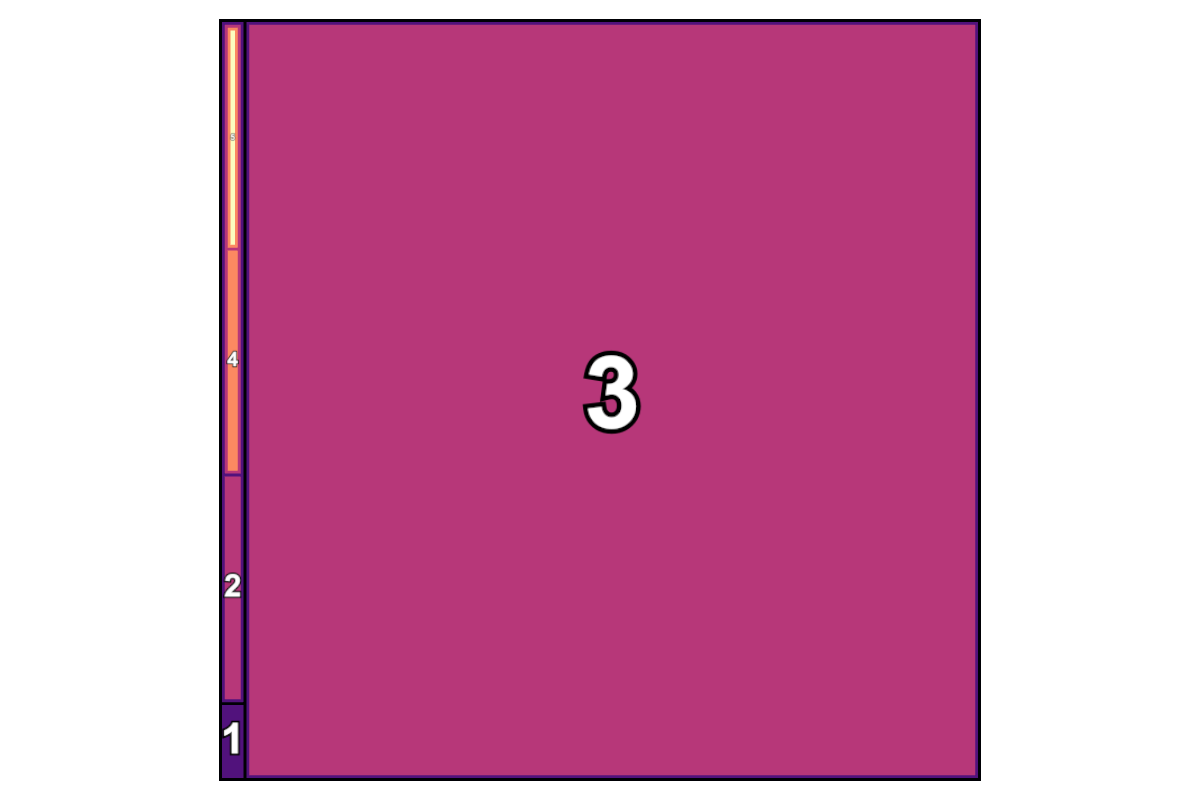
\includegraphics[width=0.8\textwidth]{images/fiveMarginArtifialMap.png}
    \caption{Treemap-Layout, generiert mit dem Squarify-Algorithmus (Abstand 5).}
    \label{fig:fiveMarginArtificialMap}
\end{figure}

\begin{figure}
    \centering
    
\includegraphics[width=0.8\textwidth]{images/tenMarginArtifialMap.png}
    \caption{Treemap-Layout, generiert mit dem Squarify-Algorithmus (Abstand 10).}
    \label{fig:tenMarginArtificialMap}
\end{figure}

Das zentrale Dilemma entsteht dadurch, dass die Kernannahme der Treemap-Algorithmen verletzt wird: Die benötigte Fläche aller Knoten einer Hierarchieebene muss vor deren Anordnung bekannt sein. Wird jedoch Fläche für Abstände benötigt, ist vorab unklar, wieviel Raum tatsächlich für jeden Knoten zur Verfügung steht. Die effektive \textit{Belegungsfläche} hängt erheblich von der jeweiligen Anordnung der Knoten ab.

Diese Problematik illustriert Abbildung \ref{fig:marginAreaDifference}. Zwei Rechtecke identischer Fläche (16 Einheiten) benötigen im Layout mit je einem Abstand von 1 eine unterschiedlich große Gesamtfläche, je nachdem, ob sie quadratisch (z.B. $4 \times 4$) oder länglich (z.B. $2 \times 8$) angeordnet sind; die zusätzliche Fläche für Abstände variiert also erheblich.

\begin{figure}
    \centering
    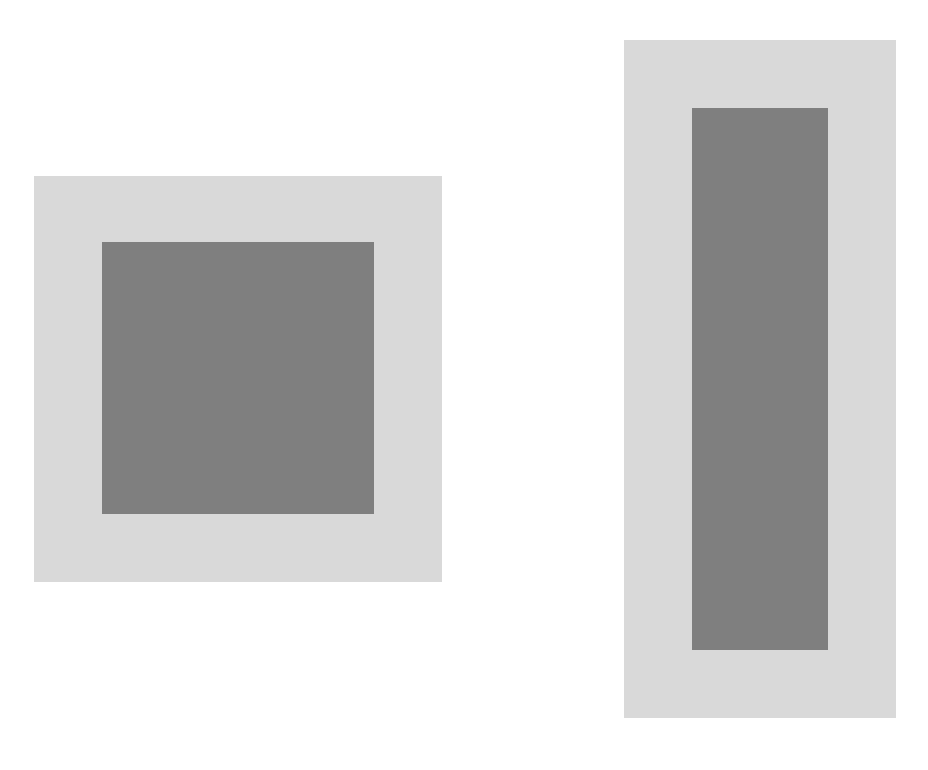
\includegraphics[width=0.8\textwidth]{images/marginArea.png}
    \caption{Zwei Rechtecke der Fläche $16$ (dunkelgrau) mit umgebendem Abstand $1$ (hellgrau): Links ($4 \times 4$) mit Gesamtfläche $25$ ($5 \times 5$), rechts ($2 \times 8$) mit $40$ ($4 \times 10$). Der jeweils notwendige Platz für Abstände hängt vom Seitenverhältnis ab.}
    \label{fig:marginAreaDifference}
\end{figure}

Dadurch entsteht ein Zirkelschluss: Das endgültige Layout kann erst berechnet werden, wenn die tatsächlich benötigte Knotenfläche (inklusive Abstände) bekannt ist. Diese Fläche hängt aber wiederum vom Layout ab. Eine triviale Lösung existiert hierfür nicht, weshalb in dieser Arbeit verschiedene Ansätze untersucht werden, um dieses Problem zu lösen (siehe Abschnitt \ref{sec:VerbesserungSquarify}).